\section{Representing Data}

\subsection{Figures}

See Figures~\ref{fig:fnCompModel}, \ref{fig:game-based_proofs} and \ref{fig:proveit_screenshot} for examples of including graphics/images as figures.
\TODO{Rule: Figures have captions below.}
\TODO{Rule: All the figures and tables must be referred to somewhere in the text.}

\begin{figure}[h] % Preferrably place figure here, not at the top/bottom of a page.
    \centering
    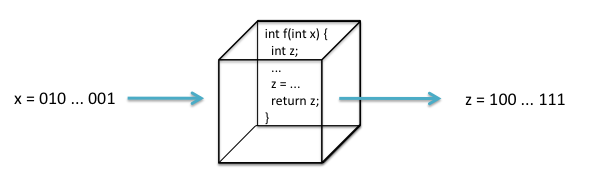
\includegraphics[width=0.8\textwidth]{computational_model_function}
    \caption{Caption for the figure.}
    \label{fig:fnCompModel}
\end{figure}

\begin{figure}[h] % Preferrably place figure here, not at the top/bottom of a page.
    \centering
    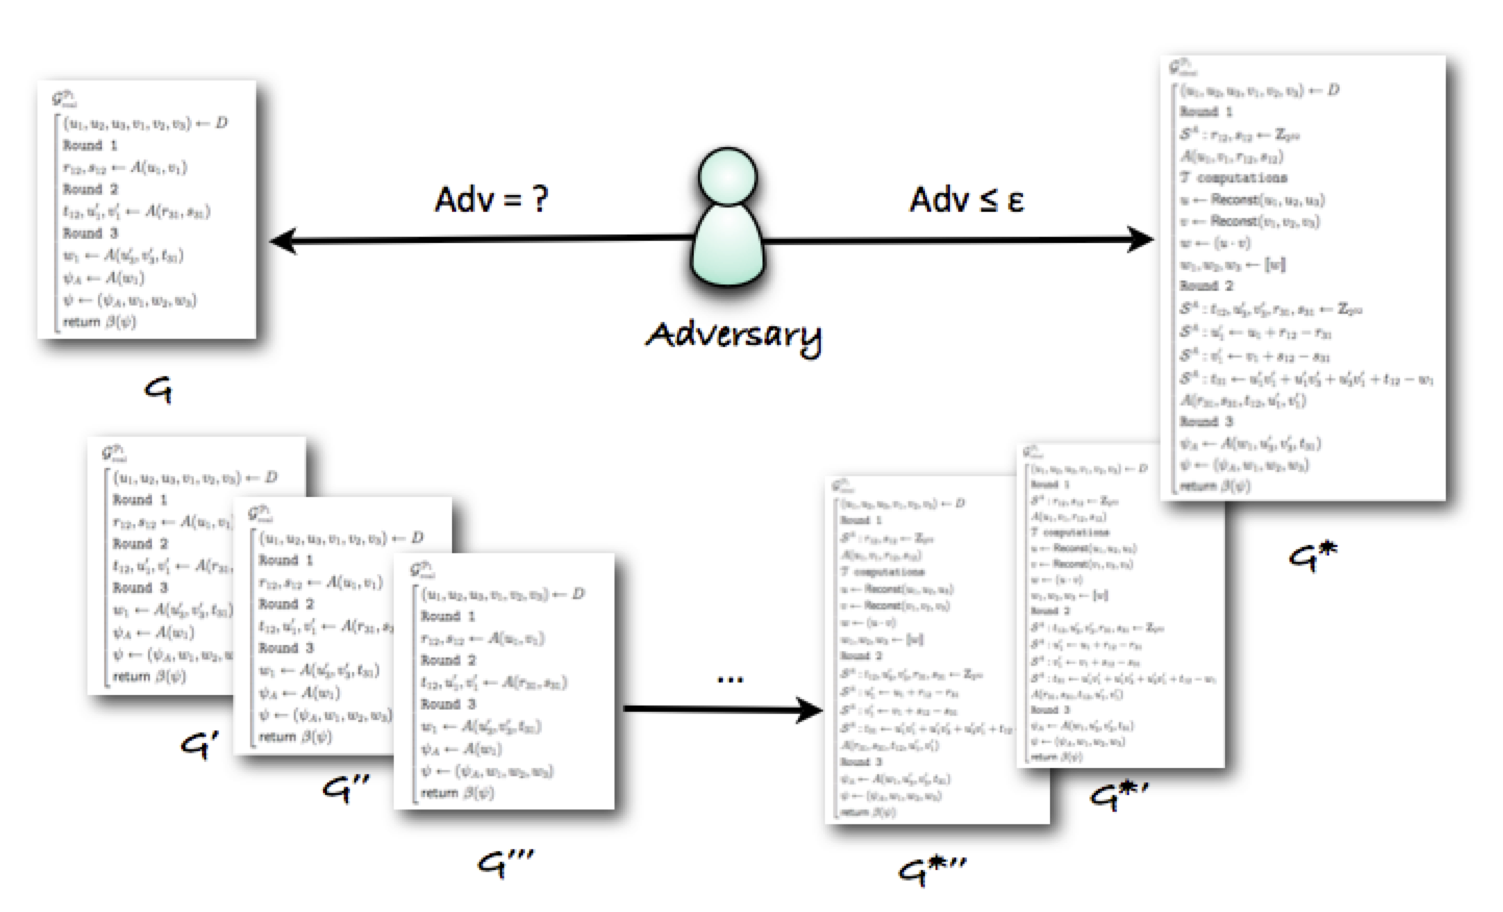
\includegraphics[width=\textwidth]{game-based_proofs}
    \caption{Cite if the figure is not yours~\cite{kamm12}.}
    \label{fig:game-based_proofs}
\end{figure}

\begin{figure}
    \centering
    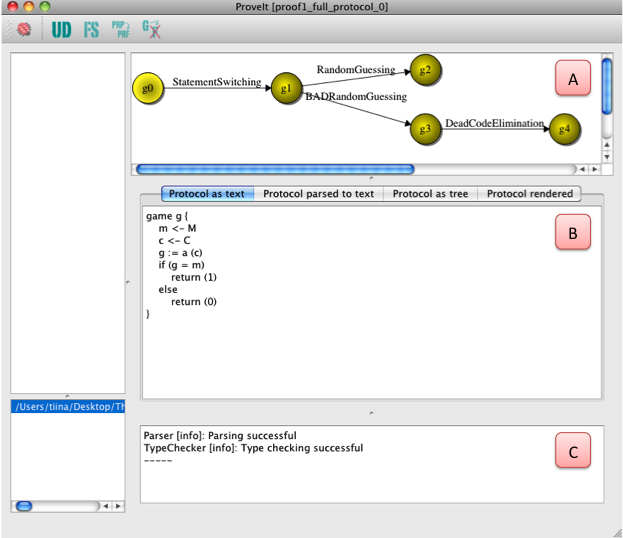
\includegraphics[width=\textwidth]{proveit_screenshot}
    \caption{Screenshot of \proveit.}
    \label{fig:proveit_screenshot}
\end{figure}

Tip: If you add a screenshot, then labeling the parts might help make the text more understandable (panel C vs bottom right part). For example:
A screenshot of \proveit can be seen in Figure~\ref{fig:proveit_screenshot}.
The user first enters the pseudocode of the initial game in panel~B.
\proveit also keeps track of all the previous games showing the progress on a graph shown in panel~A.

\begin{figure}
    \centering
    \begin{subfigure}[c]{0.45\textwidth}
        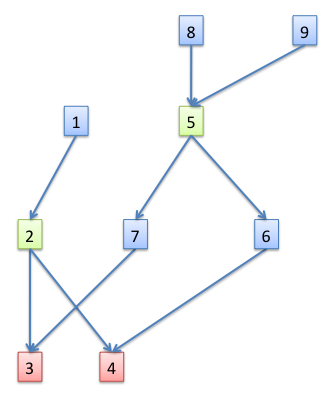
\includegraphics[width=\textwidth]{LCA_2_solutions}
        \caption{Example graph.}
        \label{fig:graph}
    \end{subfigure}
    \hfil % Add horizontal space between subfigures.
    \begin{subtable}[c]{0.3\textwidth}
        \centering
        \caption{Descendants per node.}
        \begin{tabular}{cl}
            \toprule
            Node & Decendants \\
            \midrule
            1 & 2, 3, 4 \\
            2 & 3, 4 \\
            3 & \\
            4 & \\
            5 & 3, 4, 6, 7 \\
            6 & 4 \\
            7 & 3 \\
            8 & 3, 4, 5, 6, 7\\
            9 & 3, 4, 5, 6, 7\\
            \bottomrule
        \end{tabular}
    \end{subtable}
    \caption{Example how to put two figures parallel to each other.}
    \label{fig:LCA_2_solutions}
\end{figure}

You can also use subfigures and subtables like in Figure~\ref{fig:LCA_2_solutions}.\footnote{Although you should avoid mixing subfigures and subtables like that.}


\subsection{Tables}

See Table~\ref{tab:statements} for an example of a nice and professional table that does not use vertical rules.
\TODO{Rule: Tables have captions above.}

\begin{table}
    \centering
    \caption{Statements in the \proveit language.}
    \label{tab:statements}
    \begin{tabular}{ll}
        \toprule
        Statement & Typeset Example \\
        \midrule
        assignment & $a := 5 + b$ \\
        uniform choice & $m \gets M$ \\
        function signature & $f : K \times M \to L$ \\
        \bottomrule
    \end{tabular}
\end{table}


\subsection{Lists}

Example of a numbered list:
\begin{enumerate}
    \item item one;
    \item item two;
    \item item three.
\end{enumerate}


\subsection{Math}

Variables or equations in text are surrounded by \verb|$| signs, e.g., $a$ and $x - y$.
This is a display equation:
\[
    x^2 + y^2 = z^2.
\]
This is a numbered equation:
\begin{equation}
    a + b = c + d.
    \label{eq:abcd}
\end{equation}
Multiple equations can be aligned like this:
\begin{align*} % The * means they are not numbered.
    a &= 5 \\
    b + c &= a \\
    a - 2 \cdot 3 &= \frac{5}{4}
\end{align*}


\subsection{Source code}

You can use the modern minted package to add highlighted source code like in Figure~\ref{fig:parser_exp}.

\begin{figure}
    \begin{minted}{antlr}
        expression
        : NUMBER
        | VARIABLE
        | '+' expression
        | expression '+' expression
        | expression '*' expression
        | function_name '(' parameters ')'
        | '(' expression ')'
    \end{minted}
    \caption{ANTLR grammar of arithmetic expressions.}
    \label{fig:parser_exp}
\end{figure}
